\documentclass [letterpaper, 12pt] {article}
\usepackage[margin=1in]{geometry}
\usepackage{graphicx, subcaption, ragged2e}
\usepackage{amsmath}
\usepackage{epsfig}
\usepackage{parskip}
\usepackage[utf8]{inputenc}
\usepackage[english]{babel}
\usepackage{cite}
\usepackage{float}

\graphicspath{{../Figures/}}

\begin{document}

	\begin{titlepage}
	\centering
	\vspace*{\fill}

	\vspace*{0.5cm}

	\huge\bfseries
	Data-driven Comparison of Plague Models
	
	\vspace*{0.5cm}

	\large Luke Mattfeld

	\vspace*{\fill}
	\end{titlepage}

\pagenumbering{roman}
\tableofcontents
\newpage
\pagenumbering{arabic}

\section {Abstract}

here is where one writes the abstract. An abstract abstract is the best kind of abstract

\pagebreak

\section {Introduction}

The Plague has devastated populations and greatly affected human history in its 3 major outbreaks. These outbreaks include the Justinian Plague, the Bubonic Plague, and the more recent outbreak in the 1800’s in China. [citation needed]
The driving force of the plague is the bacteria Yersinia Pestis, which manifests in 3 primary infection types: bubonic, pneumonic, and septicaemic

Bubonic plague, the most well-known, manifests in painful, swollen “Buboes” at or near the lymph nodes. It is spread through contact with the skin, in most cases insect bites. The mortality rate for untreated bubonic plague is 40-70\% \cite{ditchburn_hodgkins_2019} . Pneumonic plague, also fairly deadly, is spread through aspirated bacteria, and starts in the lungs. It is spread through aspiration in the presence of infected individuals or in an environment laiden with the bacteria. The mortality rate for untreated pneumonic plague is ~90-95\% Finally, there is a septicaemic plague which is the most deadly. Incubation for septicaemic is veryfast, and spreads fast throughout the body. Some reports said infected individuals would feel fine in the morning and be dead by evening. This had little effect on the overall epidemic when compared to the Bubonic and Pneumonic plagues, only accounting for 10-15\% of all cases of the plague since people would tend to die before they had time to develop other symptoms or methods of spreading. For this reason, the septicaemic plague will not be used in this research. The mortality rate for untreated septicaemic plague is 100\% \cite{ditchburn_hodgkins_2019}.

While historical evidence contains many details as to how the various outbreaks of the Plague have affected society, art, and culture, much less is known and is certain about the way in which the plague spread. The state of medical technology at the time has led to speculation and deductive reasoning from the available data. From this the currently accepted theory has been formed: The Bubonic plague was mostly spread through the interaction of rat and flea populations. The fleas host the disease contracted through biting a host. The fleas then are carried by the rats, which are not significantly affected by the disease. Once a carrying capacity for the rat has been reached, the flea is forced to find another host. Due to the nature of the bacteria, the digestive tract of the flea is “clogged up” (better alliteration needed) and the flee is pushed to constant biting due to hunger. The flea then regurgitates the bacteria into the many open bites. In this way the bacteria enters the new host. 

Specifically when examining the second outbreak, the poor hygienic conditions in Europe at the time, the presence of rats and fleas in and around human habitation was common. Thus, when infected rats arrived through trade routes and incoming ships, the population was quickly infected.
The exact role of the pneumonic plague is somewhat unknown. It does, under certain conditions, form from an existing case of bubonic plague, and is then spread as pneumonic from that point on. Some records of death rates are in areas and at rates which would be explained better by the spread of this pneumonic type. However, the lack of medical knowledge at the time fails us here.
This theory is partially supported by historical evidence - as sightings of sick rats were observed, and were thought to bring “bad air” which was the source of new infection. In addition ships began to be refused at many ports in Europe due to the infection they carried via the rats and sailors. [citation needed]

However Dean et. al. in a recent modeling study suggest otherwise \cite{Dean1304}. In this paper, Dean et al. investigates several mechanisms of spread likely to be responsible for historic plague events. They accomplished this by fitting the various differential models of plague spread (Rat-flea, pneumonic, and  a new human-ectoparasite model) to historical death rates. Their results suggested that the new Human-ectoparasite model better predicted the death curve over the course of the 2nd wave of the disease.

%\pagebreak
%
%\section {Background}


\pagebreak

\section {Preliminary Models}
This paper's seminal work by Dean et.\ al. \cite{Dean1304} set out to compare 3 models of
transmission: 2 for bubonic and 1 for pneumonic plague. The rat-flea model used was obtained from two papers by Keeling and Gilligan \cite{keeling_gilligan_zoonosis} \cite{keeling2000}, and going forward will be referred to as the Keeling-Gilligan model. While in the Dean work the Keeling-Gilligan rat-flea model did not perform as well as the Human-ecto model, a new rat-flea model has recently been proposed. This model developed by Oster and Lynch [citation needed], hereafter known as the Lynch-Oster model, takes a different model structure to that of Keeling and Gilligan. These models, taken from their respective papers, are as such:

\subsection {Pneumonic Model}
Direct human-to-human transmission, modeled with three differential equations. Since so few recovered from the pneumonic plague, the population follows a simple SID model
(Susceptible, Infected, Dead.):

\begin{figure}[H]
	\centering
	
\includegraphics[width=0.5\linewidth]{sid-graph.png}
	\caption{SIR Model Diagram}
\end{figure}


\begin{align}
	\frac{dS_h}{dt} &= - \beta_p \frac{S_h I_h}{N_h} \\
	\frac{dI_h}{dt} &= \beta_p \frac{S_h I_h}{N_h} - \gamma_p I_h \\
	\frac{dD_h}{dt} &= \gamma_p I_h
\end{align}


\subsection {Keeling-Gilligan Rat Model}
This model of rat-flea-human transmission is modeled with ten differential equations. Given that fleas live on the rats, they are modeled as an average number of fleas per rat H, and the number of infections fleas not on rats F:

\begin{align}
	\frac{dH}{dt} &= r_f H \left( 1 - \frac{H}{K_f} \right) \\
	\frac{dF}{dt} &= (1 - g_r) \gamma_r I_r H - d_f F
\end{align}

The Rat and Human populations follow an SIRD model (Susceptible, Infected, Recovered, Dead):

\begin{figure}[H]
	\centering
	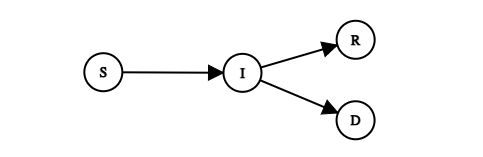
\includegraphics[width=0.65\linewidth]{sird-graph.png}
	\caption{SIRD Model Diagram}
\end{figure}

\begin{align}
	\frac{dS_j}{dt} &= - \beta_r \frac{S_j F}{N_j} \left[ 1 - e^{-aN_r} \right] \\
	\frac{dI_j}{dt} &= \beta_r \frac{S_j F}{N_j} \left[ 1 - e^{-aN_r} \right] - \gamma_j I_j \\
	\frac{dR_r}{dt} &= g_j \gamma_j I_j \\
	\frac{dD_r}{dt} &= (1 - g_j) \gamma_j I_j
\end{align}

Here, j = r, h for rats and humans respectively

In this case, the total of population j is $T_j = S_j + I_j + R_j$.

\subsection{Lynch-Oster Rat Model}

These equations govern the dynamics of the rats and fleas with logistic models:

\begin{align}
	\frac{dR_T}{dt} &= (\frac{\beta_R}{K_R})R_T(K_R-R_T)-\delta R_c \\
	\frac{dR_c}{dt} &= \alpha \frac{F_c}{F_T} (R_T-R_c)-\frac{\beta_R}{K_R}(R_T)(R_c) - \delta R_c - \gamma R_c \\
	\frac{dF_T}{dt} &= (\frac{\beta_F}{K_F})F_T(K_F-F_T)-\rho F_T  \\
	\frac{dF_c}{dt} &= \lambda \frac{R_c}{R_T} (F_T-F_c) - \rho F_c 
\end{align}

Here $R_t$ indicates the total population of rats and $R_c$ indicates the number of contaminated rats. The equations for the fleas follow similarly.

The human dynamics follow an SEIR model (Susceptible, Exposed, Infected, Recovered) where the inflow to the infected state depends on the
population density of the contaminated fleas and an interaction term for the two populations.

\begin{figure}[H]
	\centering
	
\includegraphics[width=0.75\linewidth]{seir-graph.png}
	\caption{SEIR Model Diagram}
\end{figure}

\begin{align}
	\frac{dS}{dt} &= \beta (S+R_b) - \sigma S \frac{F_c}{F_T} - \mu S \\
	\frac{dE}{dt} &= \sigma S \frac{F_c}{F_T} - \nu E - \mu E \\
	\frac{dI}{dt} &= \nu E - \phi I - rI \\
	\frac{dR_b}{dt} &= rI - \mu R_b
\end{align}



\subsection {Human-Ectoparasite Model}
Human-parasite transmission is modeled with seven differential equations.

Here, the parasite modeled is lice, which follows an SI model (Susceptible, Infected):

\begin{align}
	\frac{dS_l}{dt} &= r_l S_l \left( 1 - \frac{N_l}{K_l} \right) - \left[ \left( \beta_{low} I_{low} + \beta_{high} I_{high} \right) \frac{S_l}{N_h} \right] \\
	\frac{dI_l}{dt} &= \left[ \left( \beta_{low} I_{low} + \beta_{high} I_{high} \right) \frac{S_l}{N_h} \right] - \gamma_l I_l
\end{align}

The human population follows an $S I_l I_h R D$ model (Susceptible, Infected (low), Infected (high), Recovered, Dead):

\begin{figure}[H]
	\centering
	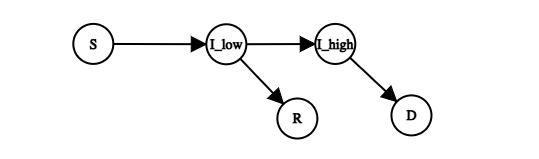
\includegraphics[width=0.75\linewidth]{siird-graph.png}
	\caption{SIIRD Model Diagram}
\end{figure}

\begin{align}
	\frac{dS_h}{dt} &= -\beta_l \frac{S_h I_l}{N_h} \\
	\frac{dI_{low}}{dt} &= \beta_l \frac{S_h I_l}{N_h} - \sigma_b I_{low} \\
	\frac{dI_{high}}{dt} &= (1-g_h) \sigma_b I_{low} - \gamma_b I_{high} \\
	\frac{dR_h}{dt} &= g_h \sigma_b I_{low} \\
	\frac{dD_h}{dt} &= \gamma_b I_{high} \\
\end{align}

This model includes terms which differentiate between high and low infectiousness of bacteria.

\pagebreak

\subsection{Parameters}
\subsubsection{Table of Parameters for existing models}
Table reconstructed from Dean et. al \cite{Dean1304}
\begin{table}[H]
\resizebox{\textwidth}{!}{%
\begin{tabular}{|c|l|l|}
\hline
\multicolumn{1}{|c|}{\textbf{Parameter}} & \multicolumn{1}{c|}{\textbf{Value}} & \multicolumn{1}{c|}{\textbf{Definition}}                                        \\ \hline
\multicolumn{1}{|l|}{\textbf{Humans}} &  &  \\
$\beta_{low}$ & U(0.001, 0.05) & Transmission rate for bubonic plague from mildly infectious humans to body lice \\
$\beta_{high}$ & U(0.001, 1) & Transmission rate for bubonic plague from highly infectious humans to body lice \\
$\beta_p$ & U(0.001, 1) & Transmission rate for pneumonic plague \\
$\beta_h$ & U(0.001, 0.2) & Transmission rate for bubonic plague from rat fleas to humans \\
$\sigma_b^{-1}$ & 8.0 (d) & Average low infectious period for bubonic plague \\
$\gamma_b^{-1}$ & 2.0 (d) & Average high infectious period for bubonic plague \\
$\gamma_p^{-1}$ & 2.5 (d) & Average infectious period for pneumonic plague \\
$\gamma_h^{-1}$ & 10.0 (d) & Average duration of infection for bubonic plague \\
$g_h$ & 0.4 & Probability of recovery from bubonic plague \\ \hline
\multicolumn{1}{|l|}{\textbf{Lice}} &  &  \\
$r_l$ & 0.11 (per d) & Natural lice growth rate \\
$K_l$ & 15.0 (per person) & Lice index at carrying capacity \\
$\beta_l$ & 0.05 & Transmission rate for bubonic plague from body lice to humans \\
$\gamma_l^{-1}$ & 3.0 (d) & Average infectious period for bubonic plague \\ \hline
\multicolumn{1}{|l|}{\textbf{Rats}} &  &  \\
$\beta_r$ & U(0.001, 1) & Transmission rate for bubonic plague from rat fleas to rats \\
$\gamma_r^{-1}$ & 5.2 (d) & Average infectious period for bubonic plague \\
$g_r$ & 0.1 & Probability of recovery from bubonic plague \\ \hline
\multicolumn{1}{|l|}{\textbf{Fleas}} &  &  \\
$r_f$ & 0.0084 (per d) & Natural flea growth rate \\
$K_f$ & 6.0 & Average number of fleas at carrying capacity \\
$d_f^{-1}$ & 5.0 (d) & Death rate of fleas \\
$a$ & 3.0/$S_r(0)$ & Searching efficiency \\ \hline
\end{tabular}%
}
\caption{U indicates the range of a uniformly distributed variable. (d) indicates days}
\end{table}


\subsubsection{Table of Parameters for the Lynch-Oster model}

\begin{table}[H]
\resizebox{\textwidth}{!}{%
\begin{tabular}{|c|l|l|}
\hline
\multicolumn{1}{|c|}{\textbf{Parameter}} & \multicolumn{1}{c|}{\textbf{Value}} & \multicolumn{1}{c|}{\textbf{Definition}}                                        \\ \hline
\multicolumn{1}{|l|}{\textbf{Humans}} &  &  \\
$\beta$ & U(0.001, 1) & Intrinsic birth rate \\
$\sigma$ & U(0.001, 1) & Chance of becoming infected from flea bite \\
$\mu$ & U(0.001, 1) & Intrinsic death rate \\
$v^{-1}$ & U(0.25, 10) (d) & Incubation period of the disease \\
$r^{-1}$ & U(1, 100) (d) & Rate of recovery from bubonic plague \\
$\phi^{-1}$ & U(1, 100) (d) & Death rate from bubonic plague \\ \hline
\multicolumn{1}{|l|}{\textbf{Rats}} &  &  \\
$\beta_R$ & U(0.1, 1) & Intrinsic birth rate for rats \\
$K_R$ & 1.5 * (init. cap) & Carrying capacity for rats \\
$\delta$ & U(0.001, 1) & Death rate from bubonic plague \\
$\alpha$ & U(0.001, 1) & Infectivity of the plague from fleas to rats \\
$\gamma$ & U(0.001, 1) & Recovery rate for rats \\ \hline
\multicolumn{1}{|l|}{\textbf{Fleas}} &  &  \\
$\beta_F$ & U(10, 100) & Intrinsic birth rate for fleas \\
$K_F$ & $6 * K_R$ & Carrying capacity for fleas \\
$\rho$ & U(0.001, 1) & Death rate from bubonic plague \\
$\lambda$ & U(0.001, 1) & Infectivity of the plague from rats to fleas \\ \hline
\end{tabular}%
}
\caption{U indicates the range of a uniformly distributed variable. (d) indicates days}
\end{table}

Here, most of the parameters for this model are uniformly distributed, since little is known about the physical associations of many of them. This provides bounds for possible values based on data (expound) [cite], while letting the specific output be determined by the fitting process.



\pagebreak

\section{Method: Markov-Chain Monte-Carlo}

The method we will use to compare the effectiveness of these models against real-world data is Markov-Chain Monte-Carlo (MCMC). MCMC is a method of fitting unknown parameters in models to data which follows these models.

\subsubsection{Markov Chains}
To understand MCMC, we must first define what a Markov Chain is. A definition given by Wolfram is:

"A Markov chain is collection of random variables ${X_t}$ (where the index t runs through 0, 1, ...) having the property that, given the present, the future is conditionally independent of the past." \cite{weisstein}

Effectively, a Markov chain models a sampling of steps in a state machine where the probability to travel from from one state to another is determined by a set of probabilities which not affected by previous states.

\begin{figure}[H]
	\centering
	\begin{subfigure}{0.5\textwidth}
		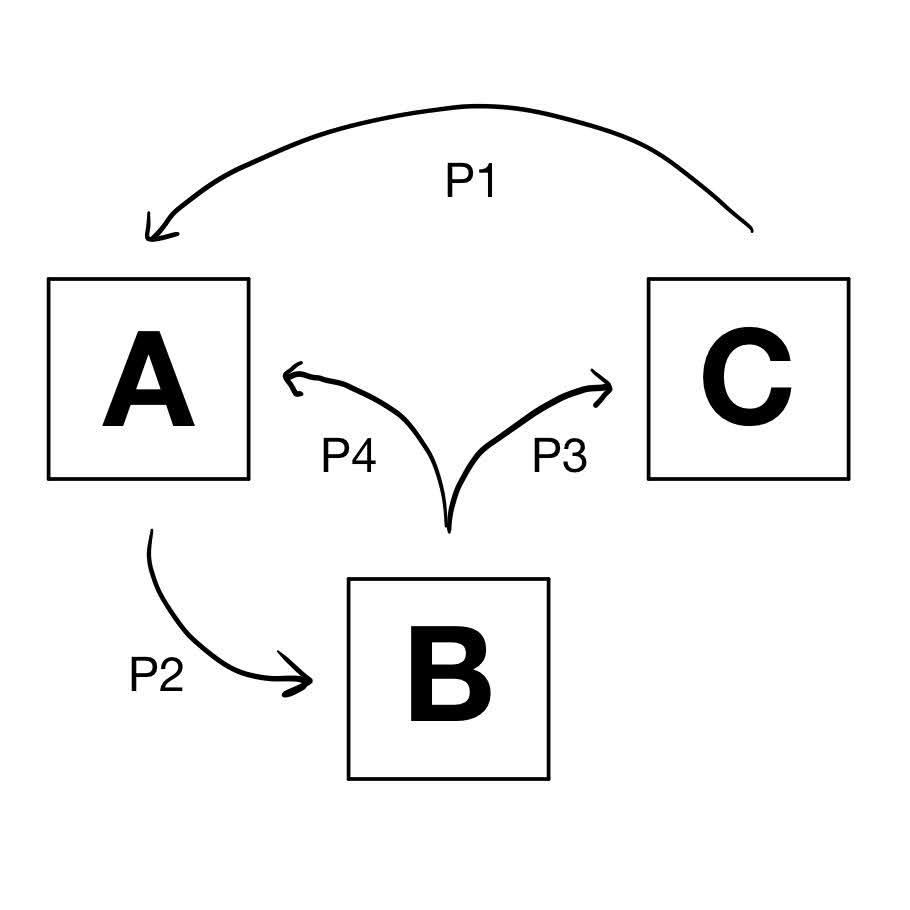
\includegraphics[width=\textwidth]{state_machine.jpg}
	\end{subfigure}
	\caption{Example diagram of a state machine where state change probabilities are determied by a set of probabilities $\{p_1, p_2, p_3, p_4\}$} 
\end{figure}

So, assuming one were to create such a state model from data obtained from some system, a markov chain based on the model would produce random variables with the same frequency as the original system data. Additionally, the chain could then be used to simulate or predict future states of the system.

\subsubsection{Mone Carlo methods}
Now, for the second part; the Monte Carlo simulation. This method is used to sample a distribution: specifically when there exists an unknown variable determined by the value of random variables having some known distribution. \cite{holmes} This can be used in simulation to achieve the probability distribution of that unknown variable, and make predictions on its value in various contexts. This kind of simulation is particularly good at long-term prediction as it "project(s) outcomes farther out in time with more accuracy" as inputs increase. \cite{ibm_cloud_2020}

\subsubsection{MCMC}

Putting these to together we get MCMC. It's a markov chain where the probabilities are calculated from local data using a Monte Carlo method.

** Explain briefly priors and posteriors, equation and bayesian method used
** Diagram of step process, explanation of burn in and what results are.



\newpage

\section {Comparison}

\subsubsection{Setup}

The known parameters for the existing models were gathered from historical data, inference of other variables, and the result of some formula. For a full derivation, see the article by Dean et. al. \cite{Dean1304}
For the unknown parameters, MCMC simulations are run to estimate based on data. For each model, we have set up the same process, and will examine the same datasets. The three data sets used here are death rates per day in Barcelona (1490), Florence (1400), and Malta (1813) [citation needed]. These were chosen from the original 9 datasets tested in Dean et al. to be representative of comparative performance. Barcelona was chosen, as it performed very well with the Human-Ecto model and was worse than the pneomonic with the existing rat model. Malta and Florence were chosen because all previous models struggled to fit well.

Each MCMC simulation took 3 samplings of 180,000 iterations with 80,000 burn-in steps and a thinning of 10. This follows the same process as was conducted by Dean et al.

In the following graphs, the black data points are recorded deaths pre day in the given data set. The red line represents the model output, and the pink outline represents the model's 95\% C.I. 

\newpage

\subsubsection{Barcelona}
For death rates in Barcelona in 1490:

\begin{center}
\textbf{Barcelona - 1490}
\end{center}
\begin{figure}[H]
	\begin{subfigure}{0.48\textwidth}
	\centering
	Pneumonic Model
	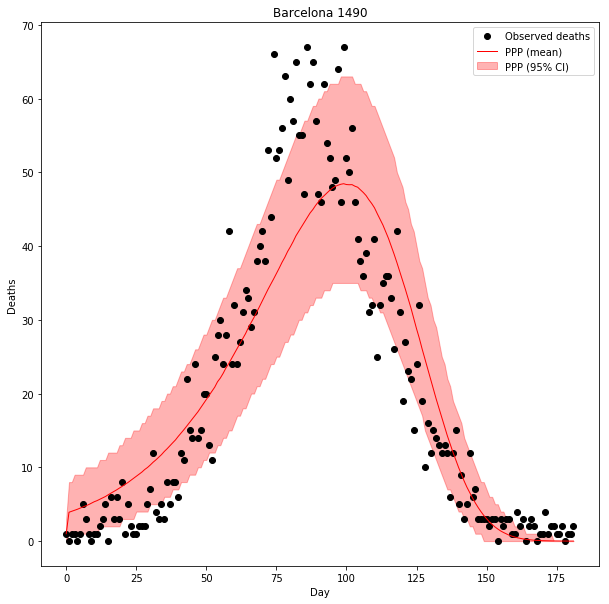
\includegraphics[width=\linewidth]{pneum_barcelona.png}
%	\caption{Pneumonic Model}
	\end{subfigure}\hspace{\fill}
	\begin{subfigure}{0.48\textwidth}
	\centering
	Keeling-Gilligan Model
	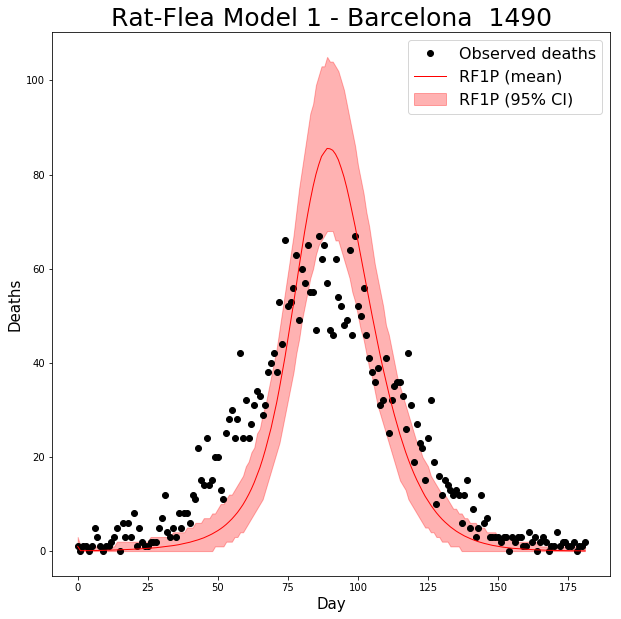
\includegraphics[width=\linewidth]{rats1_barcelona.png}
%	\caption{Keeling-Gilligan Rat Model}
	\end{subfigure}
	\begin{subfigure}{0.48\textwidth}
	\centering
	Human-Ecto Model
	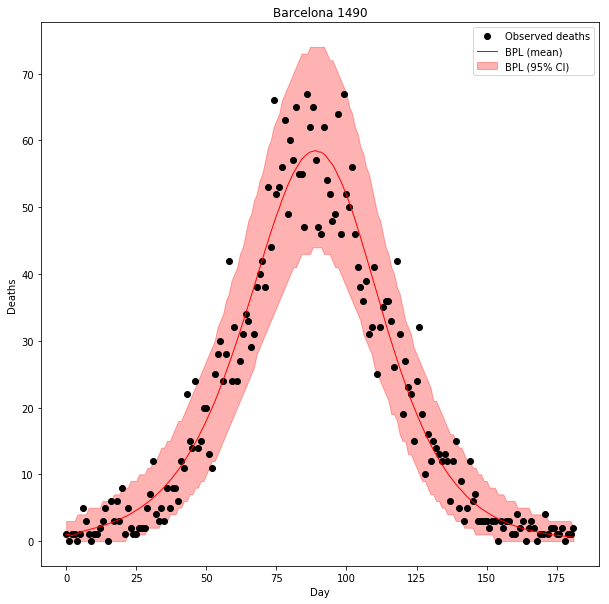
\includegraphics[width=\linewidth]{hum_ecto_barcelona.png}
%	\caption{Human-Ecto Model}
	\end{subfigure}\hspace{\fill}
	\begin{subfigure}{0.48\textwidth}
	\centering
	Lynch-Oster Model
	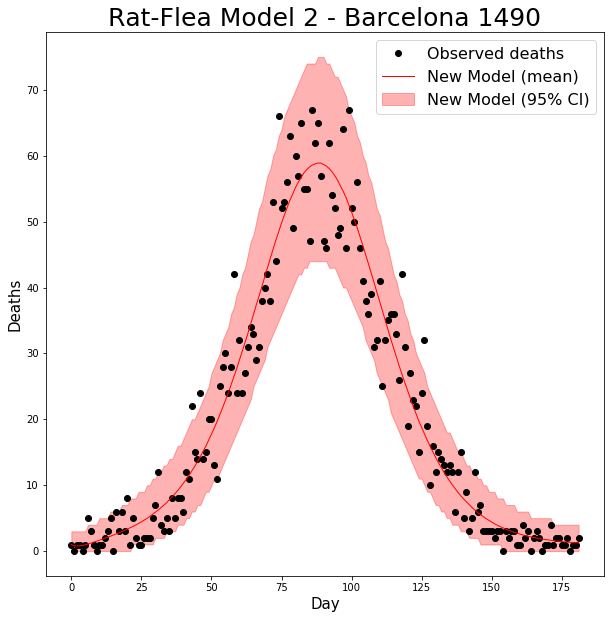
\includegraphics[width=\linewidth]{rats2_lynch_oster_barcelona.png}
%	\caption{Lynch-Oster Rat Model}
	\end{subfigure}
	\caption{Barcelona - 1490. Here, the Human-Ecto model performs the best, followed closely by the Lynch-Oster Model, and the the other two are a bit behind}
\end{figure}

\newpage
\subsubsection{Malta}
For death rates in Malta in 1813:

\begin{figure}[H]
	\begin{subfigure}{0.48\textwidth}
	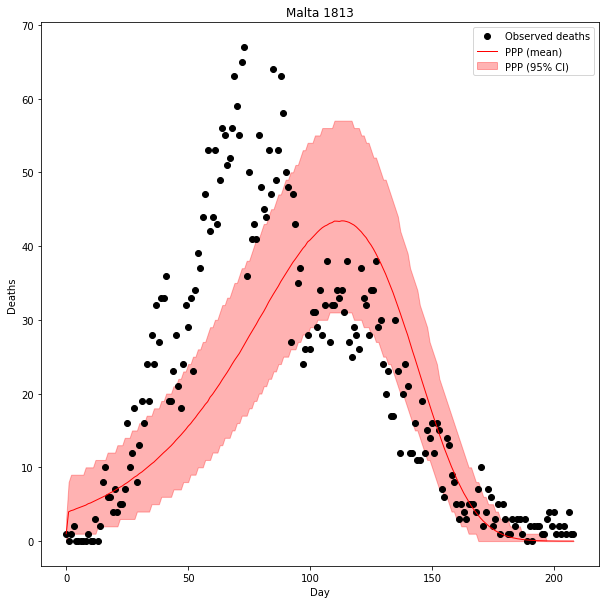
\includegraphics[width=\linewidth]{pneum_malta.png}
	\caption{Pneumonic Model}
	\end{subfigure}\hspace{\fill}
	\begin{subfigure}{0.48\textwidth}
	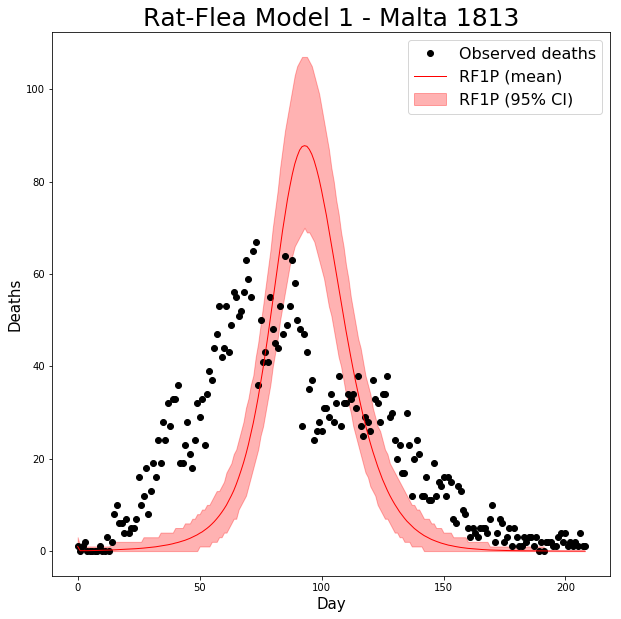
\includegraphics[width=\linewidth]{rats1_malta.png}
	\caption{Keeling-Gilligan Rat Model}
	\end{subfigure}
	\begin{subfigure}{0.48\textwidth}
	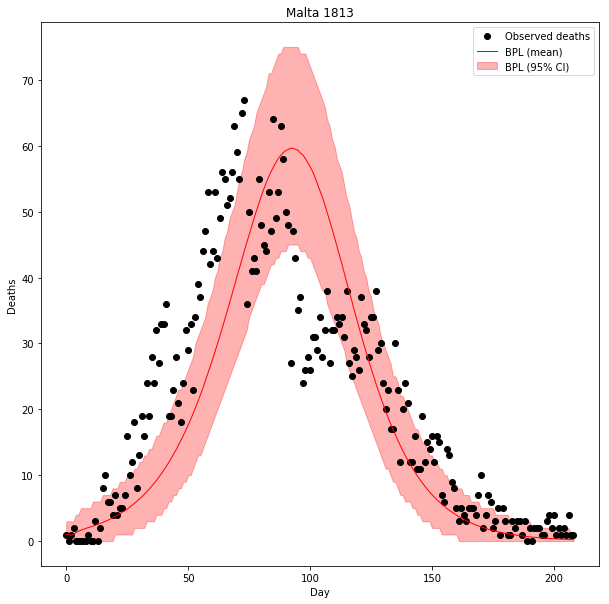
\includegraphics[width=\linewidth]{hum_ecto_malta.png}
	\caption{Human-Ecto Model}
	\end{subfigure}\hspace{\fill}
	\begin{subfigure}{0.48\textwidth}
	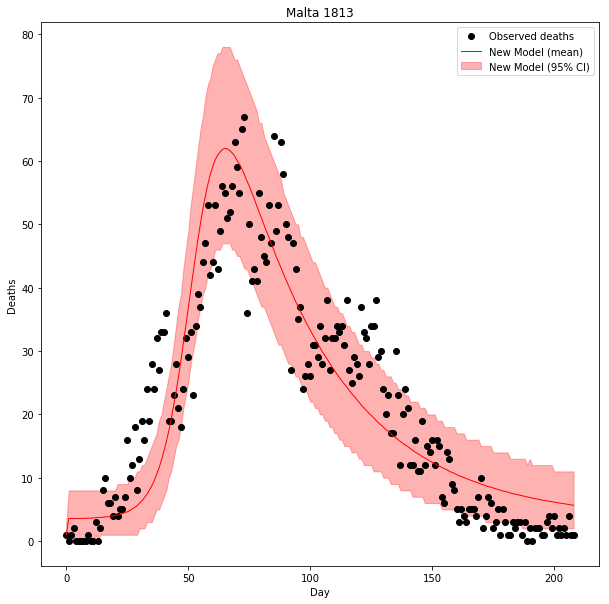
\includegraphics[width=\linewidth]{rats2_lynch_oster_malta.png}
	\caption{Lynch-Oster Rat Model}
	\end{subfigure}
	\caption{Malta - 1813. Here, the Human-Ecto model performs the best, followed by the Lynch-Oster model, then the Pneumonic model, and the Keeling-Gilligan is far behind}
\end{figure}

\newpage

\subsubsection{Florence}
For death rates in Florence in 1400:

\begin{figure}[H]
	\begin{subfigure}{0.48\textwidth}
	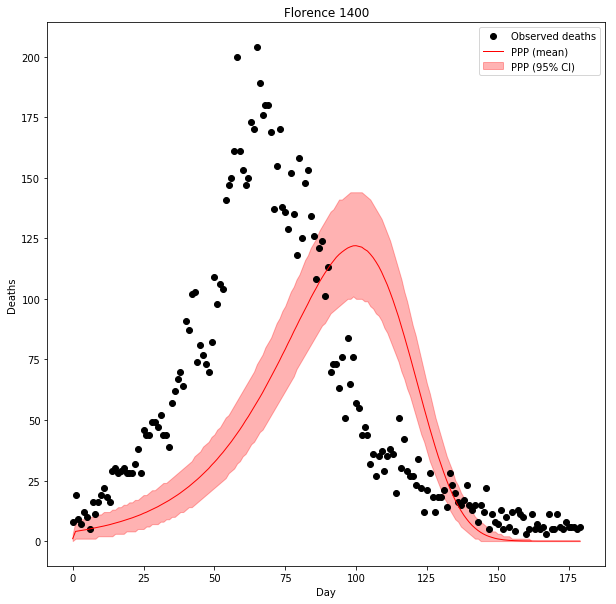
\includegraphics[width=\linewidth]{pneum_florence.png}
	\caption{Pneumonic Model}
	\end{subfigure}\hspace{\fill}
	\begin{subfigure}{0.48\textwidth}
	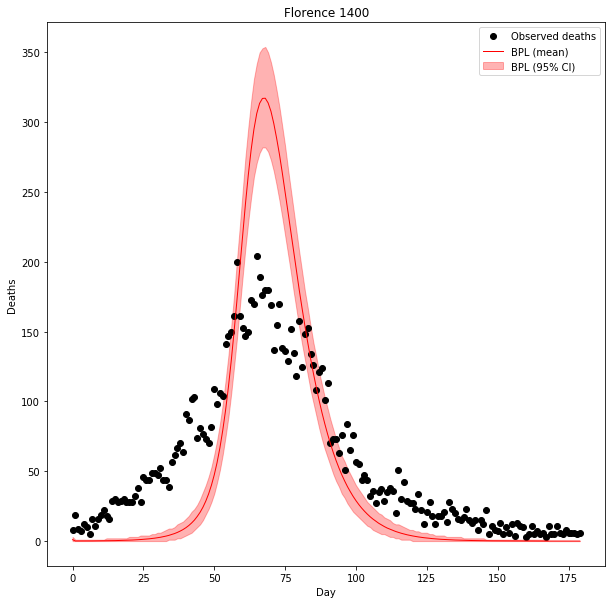
\includegraphics[width=\linewidth]{rats1_florence.png}
	\caption{Keeling-Gilligan Rat Model}
	\end{subfigure}
	\begin{subfigure}{0.48\textwidth}
	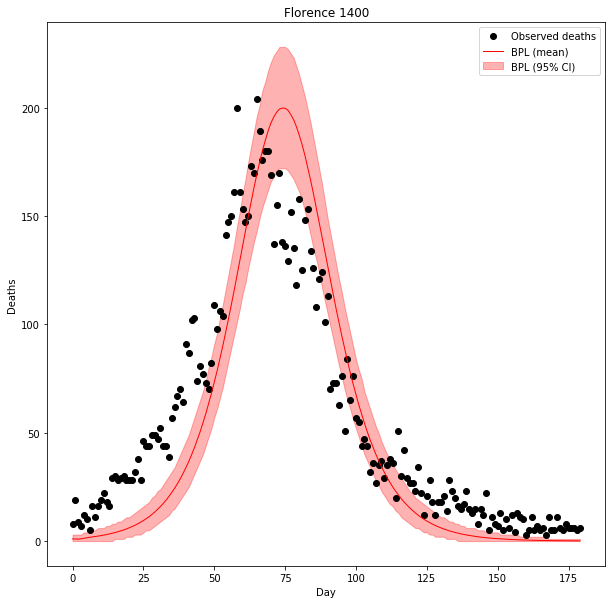
\includegraphics[width=\linewidth]{hum_ecto_florence.png}
	\caption{Human-Ecto Model}
	\end{subfigure}\hspace{\fill}
	\begin{subfigure}{0.48\textwidth}
	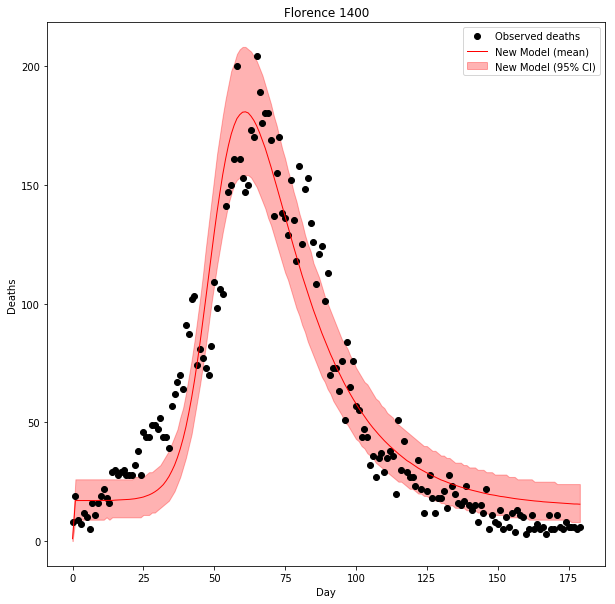
\includegraphics[width=\linewidth]{rats2_lynch_oster_florence.png}
	\caption{Lynch-Oster Rat Model}
	\end{subfigure}
	\caption{Florence - 1400. Here, the Lynch-Oster model performs best, followed by the Human-Ecto model, and the other two are quite behind}
\end{figure}

\newpage

\subsubsection{Summary}

The effectiveness of each model was measured using the Bayesian Information criterion (BIC). Here are the corresponding values for each dataset:

\begin{table}[H]
\begin{center}
\begin{tabular}{|l|l|l|}
\hline
\textbf{Dataset} & \textbf{Model}       & \textbf{BIC} \\ \hline
Barcelona        & Human-Ecto           & 1945      \\ \cline{2-3}
                 & Lynch-Oster Rat      & 2002      \\ \cline{2-3}  
                 & Pneumonic            & 2411      \\ \cline{2-3} 
                 & Keeling-Gilligan Rat & 3392       \\ \hline
Malta            & Human-Ecto           & 1945         \\ \cline{2-3} 
                 & Keeling-Gilligan Rat & 8273.8       \\ \cline{2-3} 
                 & Lynch-Oster Rat      & 2491.03      \\ \cline{2-3} 
                 & Pneumonic            & 3805.98      \\ \hline
Florence         & Human-Ecto           & 6105.4       \\ \cline{2-3} 
                 & Keeling-Gilligan Rat & 15547.45     \\ \cline{2-3} 
                 & Lynch-Oster Rat      & 2374.95      \\ \cline{2-3} 
                 & Pneumonic            & 12021.5      \\ \hline
\end{tabular}
\end{center}
\caption{BIC values per data set. A lower value indicates a better fit.}
\end{table}

\begin{table}[H]
\begin{center}
\begin{tabular}{|l|l|l|}
\hline
\textbf{Dataset} & \textbf{Model}       & \textbf{RMSE} \\ \hline
Barcelona        & Human-Ecto           & 4.9      \\ \cline{2-3} 
                 & Keeling-Gilligan Rat & 10.6      \\ \cline{2-3} 
                 & Lynch-Oster Rat      & 2002.4       \\ \cline{2-3} 
                 & Pneumonic            & 8.1       \\ \hline
Malta            & Human-Ecto           & 7.4         \\ \cline{2-3} 
                 & Keeling-Gilligan Rat & 17.6       \\ \cline{2-3} 
                 & Lynch-Oster Rat      & 7.8      \\ \cline{2-3} 
                 & Pneumonic            & 10.0      \\ \hline
Florence         & Human-Ecto           & 15.6       \\ \cline{2-3} 
                 & Keeling-Gilligan Rat & 32.7     \\ \cline{2-3} 
                 & Lynch-Oster Rat      & 16.9      \\ \cline{2-3} 
                 & Pneumonic            & 31.3      \\ \hline
\end{tabular}
\end{center}
\caption{RMSE values per data set. A lower value indicates a better fit.}
\end{table}



Overall, the Lynch-Oster model performed quite well. In each case, it was a better fit than the pneumonic and Keelin-Gilligan rat model. It performed about on par with the Human-Ecto model in Barcelona, and outperformed it in Florence.

\newpage

\section {Discussion}

While there is no clear winner when looking at the Ecto-Parasite and the Lynch-Oster models for plague spread, it's clear the new rat model brings solid evidence that the rat-based plague interpretation is certainly plausible. This calls for additional testing against new data.

As part of this, there is also more work that could be done in the fitting process. Currently, each model is run independently in Jpyter notebooks with most of the fitting process copied. This is adapted from the methods used in Dean et al. It would be beneficial for future model fitting to streamline the process to allow easily swapping out models, data, and graphing styles. This would allow researchers to quickly test the efficacy of developing new models against existing ones, and come up with better comparisons.


\pagebreak

\bibliography{References.bib}
\bibliographystyle{plain}

\end{document}